% This is LLNCS.DEM the demonstration file of
% the LaTeX macro package from Springer-Verlag
% for Lecture Notes in Computer Science,
% version 2.4 for LaTeX2e as of 16. April 2010
%
\documentclass{llncs}

% allows for temporary adjustment of side margins
\usepackage{chngpage}

% just makes the table prettier (see \toprule, \bottomrule, etc. commands below)
\usepackage{booktabs}

\usepackage[utf8]{inputenc}

% footnotes
\usepackage{scrextend}

% URL handling
\usepackage{url}
\urlstyle{same}

% Todos
%\usepackage[colorinlistoftodos]{todonotes}
%\newcommand{\ke}[1]{\todo[size=\small, color=orange!40]{\textbf{Kai:} #1}}
%\newcommand{\tb}[1]{\todo[size=\small, color=green!40]{\textbf{Thomas:} #1}}


%\usepackage{makeidx}  % allows for indexgeneration

%\usepackage{amsmath}
\usepackage{amsmath, amssymb}
\usepackage{mathabx}

% monospace within text
\newcommand{\ms}[1]{\texttt{#1}}

% examples
\usepackage{fancyvrb}
\DefineVerbatimEnvironment{ex}{Verbatim}{numbers=left,numbersep=2mm,frame=single,fontsize=\scriptsize}

\usepackage{xspace}
% Einfache und doppelte Anfuehrungszeichen
\newcommand{\qs}{``} 
\newcommand{\qe}{''\xspace} 
\newcommand{\sqs}{`} 
\newcommand{\sqe}{'\xspace} 

% checkmark
\usepackage{tikz}
\def\checkmark{\tikz\fill[scale=0.4](0,.35) -- (.25,0) -- (1,.7) -- (.25,.15) -- cycle;} 

% Xs
\usepackage{pifont}

% Tabellenabstände kleiner
\setlength{\intextsep}{10pt} % Vertical space above & below [h] floats
\setlength{\textfloatsep}{10pt} % Vertical space below (above) [t] ([b]) floats
% \setlength{\abovecaptionskip}{0pt}
% \setlength{\belowcaptionskip}{0pt}

\usepackage{tabularx}
\newcommand{\hr}{\hline\noalign{\smallskip}} % für die horizontalen linien in tabellen

% Todos
\usepackage[colorinlistoftodos]{todonotes}
\newcommand{\ke}[1]{\todo[size=\small, color=orange!40]{\textbf{Kai:} #1}}
\newcommand{\tb}[1]{\todo[size=\small, color=green!40]{\textbf{Thomas:} #1}}
\newcommand{\er}[1]{\todo[size=\small, color=red!40]{\textbf{Erman:} #1}}
\newcommand{\an}[1]{\todo[size=\small, color=blue!40]{\textbf{Andy:} #1}}

\newenvironment{table-1cols}{
  \scriptsize
  \sffamily
  \vspace{0.3cm}
  \begin{tabular}{l}
  \hline
  \textbf{Requirements} \\
  \hline

}{
  \hline
  \end{tabular}
  \linebreak
}

\newenvironment{table-2cols}{
  \scriptsize
  \sffamily
  \vspace{0.3cm}
  \begin{tabular}{l|l}
  \hline
  \textbf{Requirements} & \textbf{Covering DSCLs} \\
  \hline

}{
  \hline
  \end{tabular}
  \linebreak
}

\newenvironment{complexity}{
  \scriptsize
  \sffamily
  \vspace{0.3cm}
  \begin{tabular}{l|l}
  \hline
  \textbf{Validation Type} & \textbf{Complexity} \\
  \hline

}{
  \hline
  \end{tabular}
  \linebreak
}

\newenvironment{DL}{
  \scriptsize
  \sffamily
  \vspace{0.3cm}
  \begin{tabular}{l}

}{
  \end{tabular}
  \linebreak
}

\newenvironment{evaluation}{
  \scriptsize
  \sffamily
  \vspace{0.3cm}
  \begin{tabular}{l|c|c|c|c|c|c}
  \hline
  \textbf{constraint} & \textbf{DSP} & \textbf{OWL2-DL} & \textbf{OWL2-QL} & \textbf{ReSh} & \textbf{ShEx} & \textbf{SPIN} \\
  \hline

}{
  \hline
  \end{tabular}
  \linebreak
}

\newenvironment{user-fiendliness}{
  \scriptsize
  \sffamily
  \vspace{0.3cm}
  \begin{tabular}{l|c|c|c|c|c}
  \hline
  \textbf{criterion} & \textbf{DSP} & \textbf{OWL2} & \textbf{ReSh} & \textbf{ShEx} & \textbf{SPIN} \\
  \hline

}{
  \hline
  \end{tabular}
  \linebreak
}

\setcounter{secnumdepth}{5}

\begin{document}

%
%
\title{RDF Validation}
\subtitle{Classification of Constraint Languages According to Expressivity, Complexity, and User-Friendliness}
%
\titlerunning{XXXXX}  % abbreviated title (for running head)
%                                     also used for the TOC unless
%                                     \toctitle is used
%
\author{Thomas Bosch\inst{1} \and Erman Acar\inst{2} \and Andreas Nolle\inst{3} \and Christian Meilicke\inst{2} \and Kai Eckert\inst{2}}
%
\authorrunning{XXXXX} % abbreviated author list (for running head)
%
%%%% list of authors for the TOC (use if author list has to be modified)
\institute{GESIS – Leibniz Institute for the Social Sciences, Germany\\
\email{thomas.bosch@gesis.org},\\ 
\and
University of Mannheim, Germany \\
\email{\{christian,erman,kai\}@informatik.uni-mannheim.de} 
\and
Albstadt-Sigmaringen University, Germany \\
\email{nolle@hs-albsig.de}
}

\maketitle              % typeset the title of the contribution

\begin{abstract}
\textcolor{red}{ToDo}

\keywords{RDF Validation, RDF Constraints, OWL 2 QL, OWL 2 DL, Reasoning, RDF Validation Requirements, Linked Data, Semantic Web}
\end{abstract}
%

%\section{Possible Titles}
%
%keywords as part of the title
%
%\begin{itemize}
	%\item Classification of Constraint Languages 
	%\item Expressivity
	%\item Complexity
	%\item user-friendliness
	%\item RDF Validation
	%\item reasoning
	%\item Choosing Your RDF Constraint Language According to Expressivity, Complexity, and User-Friendliness
	%\item OWL 2 as Constraint Language for RDF Validation
	%\item Classification of RDF Validation Constraint Languages According to Expressivity, Complexity, and User-Friendliness 
	%\item RDF Validation - Classification of Constraint Languages According to Expressivity, Complexity, and User-Friendliness 
	%\item RDF Validation - Effects on Complexity with and without OWL 2 Reasoning
%\end{itemize}

\tb{I think we should replace DSCL by constraint language. DSCL disturbs the flow of reading. What do you think?}

\section{Introduction}

For many RDF applications, the formulation of constraints and the automatic validation of data according to these constraints is a much sought-after feature. 
In 2013, the W3C invited experts from industry, government, and academia to the RDF Validation Workshop\footnote{\url{http://www.w3.org/2012/12/rdf-val/}}, 
where first use cases have been presented and discussed. 
Two WGs, that follow up on this workshop and address RDF constraint formulation and validation, are established in 2014: 
the W3C RDF Data Shapes WG\footnote{\url{http://www.w3.org/2014/rds/charter}} and the DCMI RDF Application Profiles WG\footnote{\url{http://wiki.dublincore.org/index.php/RDF-Application-Profiles}}. 

Bosch and Eckert \cite{BoschEckert2014} initiated a database on RDF validation requirements, which is intended to be a way to collect case studies, use cases and especially requirements regarding RDF validation collaboratively and in a structured form.
The comprehensive, continuously maintained and extended database, which is openly available at \url{http://purl.org/net/rdf-validation}, is used to evaluate and to compare several existing solutions for RDF constraint formulation and validation. 
The requirements are classified to provide a high-level view on different solutions and to facilitate a better understanding of the problem domain \cite{BoschEckert2014}.  

There are multiple domain-specific constraint languages (DSCLs) having different syntaxes and semantics which can be used to express RDF constraints like at-least restrictions.
The most promising DSCLs are 
the SPARQL Inferencing Notation (SPIN)\footnote{\url{http://spinrdf.org/}}, 
the Web Ontology Language (OWL 2)\footnote{\url{http://www.w3.org/TR/owl2-syntax/}}, 
Shape Expressions (ShEx)\footnote{\url{http://www.w3.org/Submission/shex-primer/}}, 
Resource Shapes (ReSh)\footnote{\url{http://www.w3.org/Submission/shapes/}}, 
and Description Set Profiles (DSP)\footnote{\url{http://dublincore.org/documents/2008/03/31/dc-dsp/}}.
However, there is no single standard DSCL to express any constraint for each purpose.
The choice depends on the individual use case.

\section{Motivation}
Despite the huge diversity to formulate constraints and validate them on RDF data, most of the DSCLs require the major shortcoming of redundancy. For illustration, consider e.g., the existential restriction \ms{Jedi $\sqsubseteq$ $\exists$ hasJediWaepon . JediWeapon} that stated that every Jedi has at least one Jedi weapon. Furthermore, we know that Luke is a Jedi (\ms{Jedi(Luke)}) having a blue laser sword (\ms{hasLaserSword(Luke, BlueLaserSword)}. Since all of the DSCLs are based on the closed-world assumption (CWA) and as long as it isn't explicitly defined that a blue laser sword is a Jedi weapon (\ms{JediWeapon(BlueLaserSword)}), the existential restriction causes a constraint violation.

But if we express the mentioned constraints in OWL and apply a reasoner before the proper constraint validation is performed, we won't get a constraint violation because all implicit statements like a blue laser sword is a Jedi weapon (\ms{JediWeapon(BlueLaserSword)}) will be inferred. At a first glance, using OWL as constraint language the shortcoming of redundancy is solved. However, on closer consideration OWL is by default an insufficient choice because OWL is in contrast based on the open-world assumption (OWA), i.e. a statement cannot be inferred to be false on the basis of failures to prove it. 
This semantics is suitable for the distributed knowledge representation scenarios on the Semantic Web, 
where usually the knowledge about the domain comes from distributed
sources and a complete knowledge about the domain cannot be assumed, 
but makes it difficult to use OWL for RDF validation.
Additionally, in OWL we have the non-unique name assumption (nUNA) whereas RDF validation requires that different names represent different objects (also known as unique name assumption (UNA)).
This ambiguousness in semantics is one of the main reasons why OWL has not been adopted as standard DSCL for RDF validation in the past. 

Let us address these opposites via an example. Consider e.g., the following definition of the knowledge base $\mathcal{K}$:
\begin{eqnarray*}
\mathcal{K} &=  & \{\ms{Person} \sqsubseteq \exists \ms{hasFather.Person}, \\
 &&(\ms{funct (hasFather)}),\\
 && \ms{Person(Anakin)},\\
 && \ms{Person(Luke)},\\
 && \ms{hasFather(Luke, Anakin)},\\ 
 && \ms{hasFather(Luke, Shmi)}\}
\end{eqnarray*}

In case of the OWA, we infer that $\ms{Anakin}$ has a father that is a $\ms{Person}$, but we do not know him, so $\mathcal{K}$ is consistent. In CWA however, the constraint needs to be satisfied only by named individuals which yields in return of a constraint violation. We can further observe that there is a clash caused by the functional role $\ms{hasAncestor}$ and the UNA. However, in OWA there is no UNA by default, therefore the reasoning will conclude that $\ms{Anakin}$ is the same individual as \ms{Shmi} ($\ms{Anakin} \equiv \ms{Shmi}$). Notice that this is not a problem if we add UNA to the OWA, like in the \textit{DL-Lite} family \cite{Calvanese2007,Artale2009} which is the basis for OWL 2 QL.

If we follow the principle of adopting the UNA to OWL and performing contraint validation after some reasoning, the opposites of OWA in OWL and CWA in constraint validation doesn't affect each other, because missing assertions like in the example mentioned above will cause still some constraint violations but the implicit knowledge is even considered on constraint validation.

\tb{maybe next paragraph in front}

OWL is based on a knowledge representation formalism with different complexity, but is created as a language which can be seen as a constraint language.
Constraint validation does not appear to be part of the services provided by OWL.  
This has lead to claims that OWL cannot be used for constraint validation. 
and there are long and controversial discussions\footnote{\url{http://lists.w3.org/Archives/Public/public-data-shapes-wg/}, \url{https://www.jiscmail.ac.uk/cgi-bin/webadmin?A0=dc-architecture}} in the W3C and DCMI WGs if OWL should be used for RDF validation.
OWL is an instantiation of a high-level and very expressive DSCL with a compact human-readable syntax.
OWL is a language that many people already know.
In practice, many people use RDFS and OWL constructs to tell other people and applications about how valid instances should be created.
Normally, RDF documents follow the structure of RDFS/OWL ontologies. 
Thus, part of those declarations will be defined anyway and can therefore be reused for validating these RDF documents.

%The standard semantics of OWL is:
%
%\begin{itemize}
	%\item Open World Assumptions (OWA): a statement cannot be inferred to be false on the basis of failures to prove it.
  %\item non-Unique Name Assumptions (nUNA): two different names may refer to the same object.
%\end{itemize}
%
%This semantics is suitable for the distributed knowledge representation scenarios on the Semantic Web, 
%where usually the knowledge about the domain comes from distributed
%sources and a complete knowledge about the domain cannot be assumed, 
%but makes it difficult to use OWL for RDF validation.

%Although, most people don’t care about open world semantics, 
%ambiguousness is one of the main reasons why OWL has not been adopted as standard DSCL for RDF validation in the past. 
%When OWL would be used assuming both OWA (for reasoning) and CWA (for constraint validation),
%it would be somewhat confusing to have two completely different semantics for OWL.
%On the other hand, OWL constraints could be interpreted either with the OWA to support open
%world reasoning, and exactly the same piece can also be interpreted in closed world
%applications as a constraint. 

You can't easily use OWL to even do cardinality checking. 
For example, suppose you assert that \ms{hasFather} is a functional property, and you have the triples \ms{Luke hasFather Anakin} and \ms{Luke hasFather Darth}.
An OWL reasoner will invoke the nUNA to infer that \ms{Anakin owl:sameAs Darth}.

Therefore, the semantics for RDF validation is Closed World Assumption (CWA) and the Unique Name Assumption.
 
As for an area where OWA is problematic, one need look no further than
FRBRer ontology is clearly designed using OWL constraints
(which I prefer to call "axioms" to avoid confusion) in a closed world
way. The definitions are quite strict, with all classes disjoint each
other, such that, using reasoning in the OWL, any FRBRer data will be
inconsistent with data not using that exact set of axioms. 
http://svn.aksw.org/papers/2014/WWW\_Databugger/public.pdf

%\tb{Andy, we want to use only star wars examples in our paper. We need 1 example showing the differences between OWA / CWA and /UNA / nUNA. You may reuse star wars examples which are already in the paper.}

Let us address the CWA vs. OWA via an example. Consider the knowledge base  $\mathcal{K} = \{\ms{Person} \sqsubseteq \exists \ms{hasAncestor.Person}, \ms{Person(Luke)}\}$. In case of OWA, we know that $\ms{Luke}$ has $\ms{Ancestor}$, but we do not know all of them. Notice that $\mathcal{K}$ is consistent. In CWA however, the constraint needs to be satisfied only by named individuals which yields in return some validation errors.\\
Consider the following case in CWA. 
\begin{eqnarray*}
\mathcal{K} &=  & \{\ms{Person} \sqsubseteq \exists \ms{hasAncestor.Person}, \\
 &&(\ms{funct }  \ms{hasAncestor}),\\  && \ms{Person(Luke)},\\ && \ms{hasAncestor(Luke, Anakin)},\\  && \ms{hasAncestor(Anakin, Shmi)}\}
\end{eqnarray*}

\noindent Now, observe that there is a clash because of the functional role $\ms{hasAncestor}$ and the UNA. However, in OWA there is no UNA by default, therefore the reasoning will conclude that  $\ms{Anakin}$ to be the same individual with $\ms{Shmi (Anakin} \equiv \ms{Shmi}$). Notice that this is not a problem if we add UNA to the OWA, like in the \textit{DL-Lite} family.
Another point is that, if we perform RDF validation without reasoning, we will get a further clash: $\ms{Anakin}$ is not defined to be a $\ms{Person}$. On the other hand, if we do the validation after the reasoning, then there is no clash since $\ms{Person(Anakin)}$ is inferred. 

%\begin{itemize}
	%\item explain why specific OWL 2 constructs could be used for RDF validation 
	%\item explain why specific OWL 2 constructs should not be used for RDF validation
%\end{itemize}

Reasoning makes sense before actually validating constraints.
Reasoning, which is the core service provided by OWL,
and constraint validation are very closely related. 
Reasoning is the process of determining what follows from what has been
stated.  Reasoning ranges from simple (students are people, John is a
student, therefore John is a person) to the very complex. Reasoning can
also recognize impossibilities (students are people, John is a student, John
is not a person, therefore there is a contradiction). 
It both should be possible: (1) constraint validation with reasoning and (2) constraint validation without reasoning. 

Reasoning may be a pre validation step to infer triples resolving constraint violations.
According to the existential restriction \ms{Jedi $\sqsubseteq$ $\exists$ hasJediWaepon . JediWeapon} every Jedi has at least one Jedi weapon.
Luke is a Jedi (\ms{Jedi(Luke)}) having a blue laser sword (\ms{hasLaserSword(Luke, BlueLaserSword)}.
As it is not defined that laser swords are Jedi weapons and as Luke is a Jedi, the existential restriction causes a constraint violation. 
This constraint violation is not raised when we define that laser swords are Jedi weapons (\ms{hasLaserSword $\sqsubseteq$ hasJediWaepon} ) 
and \ms{hasLaserSword} is a sub-property of \ms{hasJediWeapon} (\ms{LaserSword $\sqsubseteq$ JediWeapon}).

It makes also sense to perform reasoning to infer triples for which constraints are validated.
The existential restriction \ms{Jedi $\sqsubseteq$ $\exists$ hasLaserSword . LaserSword} forces Jedis to have at least one laser sword.
The existential restriction is not checked for the triple \ms{YediMaster(Yoda)}, as \ms{Yoda} is a \ms{JediMaster} and not a \ms{Jedi} as well.
If, however, our knowledge base contains the axiom \ms{JediMaster $\sqsubseteq$ Jedi}, the triple \ms{Jedi(Yoda)} is inferred and the existential restrictions is validated for the individual \ms{Yoda}, raising a constraint violation if a triple such as \ms{hasLaserSword(Yoda, GreenLaserSword)} is not included in the knowledge base. 

\textcolor{red}{example}

%With regard to typing, W3C is assuming (AFAIK) that all types will be
%explicit in the instance data - for the purposes of validation. There is
%nothing, however, to prevent an application from running reasoning prior
%to validation to add inferred triples to the data being validated. But
%the general feeling right now is that validation acts on instance data
%without requiring that the validator apply reasoning in order to do so.

%Nehmen wir nun an, dass dein Framework welches entsprechende SPARQL Queries generiert diese auf einem SPARQL Endpoint evaluiert der zu der vorliegenden Ontologie bzw. des darin verwendeten OWL 2 Profils das entsprechende Entailment Regime realisiert, wären die zurückgegebenen Resultsets vollständig. Wie das Entailment Regime im Endpoint realisiert ist, also durch Query Rewriting oder durch Vervollständigung der ABox, ist dabei irrelevant.
%
%Wie allerdings bspw. in 
%\url{https://www.uni-ulm.de/fileadmin/website_uni_ulm/iui.inst.090/Lehre/WS_2011-2012/SemWebGrundlagen/LectureNotes.pdf}
%auf Seite 51 veranschaulicht, ist die Komplexität des Reasoning abhängig von der zugrunde gelegten Sprache und kann daher nur in bestimmten Fällen effizient durchgeführt werden. Wie in unserem letzten Paper beschrieben zielt unter anderem die Definition von DL-Lite gerade darauf ab Reasoning Aufgaben und Query Answering effizient zu ermöglichen und ist Grundlage des OWL 2 QL Profils. Nun ist allgemein bekannt, dass die logische Konsistenz für diese Art von Sprachen effizient geprüft werden kann. 
%
%Allerding wäre wie bspw. in 
%\url{http://www.aifb.kit.edu/images/d/d2/2005_925_Haase_Consistent_Evol_1.pdf} beschrieben auch eine sogenannte 'User-defined Consistency' denkbar. Genau an dieser Stelle könnten wir ansetzen.

%\textbf{Ideas}
%
%\begin{itemize}
	%\item RDF validation using OWL 2 QL reasoning by SPARQL query expansion
	%\item if using OWL 2 DL as constraint language or using constraints equivalent to OWL 2 QL you can use reasoning 
	%\item reasoning can also be executed using SPARQL query expansion.
	%\item reasoning not executing using reasoner
%\end{itemize}

%\begin{itemize}
	%\item complete with reasoning | OW
	%\item complete without reasoning | CW
	%\item there is no query rewriting mechanism for OWL 2, just for OWL 2 QL
%\end{itemize}

\textcolor{red}{high-level description of expressivity}

\textcolor{red}{
\begin{itemize}
  \item why is expressivity important for the paper?
	\item expressivity of query languages like SPARQL?
	\item expressivity of OWL 2 QL and OWL 2 DL?
	\item how is expressivity and complexity related?
\end{itemize}
}

\textcolor{red}{high-level description of complexity}

We group each RDF requirement into three complexity classes.
As case studies are linked to use cases and use cases to requirements, it is known how complex the task is to fulfill use cases and case studies.
For specific use cases, it can also be determined which of the associated requirements lead to a higher complexity class.
Imaginable is a system in which use cases can be selected which should be met for particular applications.
Then, the system determines the complexity class, can point to requirements and constraints causing a higher complexity class,
and can give hints how to rewrite the constraint in order to stay in a lower complexity class.   

Query languages such as SPARQL or Datalog are more expressive than OWL 2 QL and DL,
but the complexity of query languages is less than the complexity of OWL 2 QL and DL, because of the reasoning calculations.
For many constraints reasoning can be done, but when reasoning is not needed for validation this constraint can be reformulated as a query by a query language
leading to a lower complexity class. 
\textcolor{red}{example}
Such a complexity aware RDF validator could help people writing constraints that can be efficiently computed.
For DL, there is a web application allowing you to select the needed DL constructs in order to determine the complexity of DL reasoning\footnote{\url{http://www.cs.man.ac.uk/~ezolin/dl/}}.

As we evaluated to which extend each constraint can be expressed by the most promising five DSCLs, 
we can determine the complexity of these DSCLs as well. 

If we want to use OWL 2 for RDF validation, we have to ensure that as many requirements for formulating RDF constraints are fulfilled
and that the computational complexity to formulate these constraints is satisfying.  

\textcolor{red}{research questions and contributions needs to be adapted}

Therefore, we answer five \textbf{research questions}:
\begin{enumerate}
	\item Which constraints are expressible by DL and which are only expressible by a query language (e.g Datalog or SPARQL)?
	\item For which requirements formulating constraints the expressivity of \textit{DL-Lite}$_\mathcal{A}$ (respectively OWL 2 QL) is sufficient
	and for which requirements additional DSCLs are needed?
	\item For which constraints a priori reasoning makes sense and how does reasoning affect their validation?  
	\item What are the effects on complexity to express these constraints with and without OWL 2 QL and OWL 2 DL reasoning?
	\item What are the effects on complexity of constraints not expressible by DL but by a query language?
\end{enumerate}

The three \textbf{main contributions} of this paper are:
\begin{enumerate}
  \item We investigate the effects on complexity expressing each constraint
	\item We show that OWL 2 QL together with additional DSCLs completely satisfy all RDF validation requirements.
	\item We evaluated to which extend the five possible standard DSCLs fulfill each requirement.
\end{enumerate}

\textcolor{red}{paper organization}

\section{Expressivity and Complexity of OWL 2}

\textcolor{red}{
\begin{itemize}
	\item OWL as a high-level language with reasoning capabilities which can be used for RDF validation
\end{itemize}
}

\subsection{OWL 2 QL Reasoning}

OWL 2 profiles (or fragments in logic literature) are restricted (sublanguage) versions of OWL 2 that offer different trade-offs regarding expressivity  vs. efficiency in reasoning. There are three main  profiles of OWL 2, which are OWL 2 QL, OWL 2 RL and OWL 2 EL namely, each designed to  be useful for different purposes and application scenarios. The choice of which profile to use is purpose-specific on what to express and to perform the reasoning about. We refer reader to \cite{owl2profiles2008} for a comprehensive treatment of those profiles. 

OWL 2 QL is an OWL 2 profile which focuses on reasoning on query answering with very large size of instance data. The acronym QL stands for query language as query answering in this profile can be done by rewriting queries into a standard relational query language (also known as First-Order Rewritability). Also, conjunctive query answering can be done by using conventional relational database systems. Aiming at efficiency on working with large size data, the expressive power of the profile is quite limited as expected. As a result of this, reasoning in OWL 2 QL is highly efficient so that sound and complete conjunctive query answering can be performed in \textsc{LogSpace} in the size of the data assertions as well as  the ontology consistency and class expression subsumption can be performed in polynomial time.

OWL 2 QL is based on the \textit{DL-Lite} family of description logics, a tractable family of fragments of first-order logic \cite{Artale2009,Calvanese2007}. 
However, an important difference between the \textit{DL-Lite} family and OWL is the
unique name assumption (UNA). UNA is common in data management, therefore it is adopted in the \textit{DL-Lite} family whereas not adopted in OWL. In OWL, one uses constructs \textbf{sameAs} or \textbf{differentFrom} explicitly to state that two individuals, say  $a$ and $b$, are the \emph{same} or {different} respectively. For that reason in OWL 2 QL, any construct e.g., number restrictions or functionality constraints which can interfere with UNA and also which can cause higher complexity without the UNA, has been avoided. \an{but in \textit{DL-Lite}$_\mathcal{A}$ functionality is expressible, as far as I know there is also an extension to \textit{DL-Lite}$_\mathcal{A}$ that allows number restrictions...}

Among the members of \textit{DL-Lite} family, \textit{DL-Lite}$_\mathcal{R}$ is the one that OWL 2 QL is based on. The reason is to avoid any problematic issue which might appear in the explicit axiomatization of UNA, since  \textit{DL-Lite}$_\mathcal{R}$ in general does not require the UNA, because making this assumption has no semantic affect on a \textit{DL-Lite}$_\mathcal{R}$ ontology.

\subsection{OWL 2 DL Reasoning}

%\tb{ToDO for Erman and Andy: can you please write a short paragraph about OWL 2 DL reasoning?}

The Semantic Web ontology language OWL 2 DL\footnote{See \url{http://www.w3.org/TR/owl2-direct-semantics/}.} was standardized by
the World Wide Web Consortium (W3C) in 2009 (and updated in 2012) as a
description logic-like formalism.  OWL 2 DL has high expressivity, yet maintains  decidability for main reasoning tasks e.g., ontology satisability, 
entailment checking. The drawback of its expressive power results as a lack of computational efficiency in performance. In general, reasoning in OWL 2 DL is in \textsc{N2exptime} \cite{owl2profiles2008}. 

As a result of its expressive power, OWL 2 DL allows a large variety of sophisticated modeling capabilities for many application domains.  On the other hand, to maintain the decidability, OWL 2 DL has a numerous ways of syntactic restrictions. One example is that OWL 2 DL allows  expressing transitive properties as well as asymmetric properties, yet a property to be both transitive and asymmetric (just as ancestor relation) is not allowed. In the sequel, from RDF validation perspective, we will give some examples of constraints that remain at the outside of its scope. 

\section{Classification of RDF Constraints and DSCLs according to Expressivity, Complexity, and User-Friendliness}

\textcolor{red}{
\begin{itemize}
	\item section 3 is needed as basis for this chapter to which extend do most promising five constraint languages cover RDF validation requirements?
	\item --> then, constraint languages can also be assigned to these classes (e.g. 6 out of 30 class A requirements are covered by constraint language A --> constraint language A is also assigned to that class)
\end{itemize}
}

\textcolor{red}{at least 1 example for each class}

%We divide these constraints into three classes:
%\begin{itemize}
	%\item constraints expressible by OWL 2 QL
	%\item constraints not expressible by OWL 2 QL but by OWL 2 DL
	%\item constraints only expressible by other DSCLs
%\end{itemize}

The W3C and DCMI WGs identified in total 74 requirements to formulate RDF constraints\footnote{Two of this paper's authors are actively contributing to these WGs and the process deriving requirements from case studies and use cases is still ongoing.}.
Bosch et al.\footnote{available at: \url{https://github.com/boschthomas/rdf-validation-research/paper}} explained each requirement in detail and give at least one example for each of them represented by different DSCLs.
We added mappings to DL in order to logically underpin each requirement and in order to determine which DL constructs are needed to express each constraint.
When the DL constructs, needed to express a particular constraint, are known, the expressivity and the complexity of this constraint can be determined. 
The constraint \ms{Context-Specific Exclusive OR of Properties} (see section~\ref{sec:rdf-validation-requirements-without-reasoning-2}), for example, can generically be expressed as follows:
\begin{eqnarray*}
C \sqsubseteq (\neg A \sqcap B) \sqcup (A \sqcap \neg B) \\
A \equiv \exists a . D \\
B \equiv \exists b . E  
\end{eqnarray*}
As this constraint is a complex constraint (constructed out of multiple complex and simple constraints), 
the constraint's expressivity is calculated as the expressivity of the individual constraints used to express the complex constraint.
The DL constructs \ms{property inclusion}, \ms{complement}, \ms{intersection}, \ms{union}, and \ms{existential restriction} are used to express this constraint.  
As existential restrictions are part of OWL 2 DL reasoning, the constraint's complexity is \textsc{N2exptime}.
 
We evaluated to which extend the most promising five DSCLs fulfill each requirement.
We also evaluated if a specific requirement is covered by OWL 2 QL or if the more expressive and complex OWL 2 DL is needed \cite{BoschNolleAcarEckert2015}.

\tb{How to publish the requirements evaluation? as technical report?}

\subsection{Classification Dimension Expressivity}

There are no reserved words for expressivity of DSCLs like LOGSPACE for complexity in computational logic.
As a consequence, for the expressivity of DSCLs, we need to define our own reserved words.
As we want to be able to perform reasoning before actually validating the data, we identified four RDF validation expressivity classes, 
which we define as follows: 

\begin{itemize}
	\item \ms{Expr-R-OWL2-QL}: OWL 2 QL reasoning axioms
	\item \ms{Expr-R-OWL2-DL}: OWL 2 DL reasoning axioms
	\item \ms{Expr-R}: reasoning axioms not supported by OWL
	\item \ms{Expr-C}: constraints without reasoning
\end{itemize}

Reasoning axioms can be used for its original purpose to infer new triples out of explicitly stated triples (see section \ref{sec:rdf-validation-requirements-and-reasoning}), but also to express constraints.
If in our knowledge base it is stated that \ms{DarthVader} is a \ms{Sith} (\ms{Sith(DarthVader)}) and that Siths feel the force of the dark side (\ms{Sith $\sqsubseteq$ FeelingForceDarkSide}), it is either possible to infer that \ms{DarthVader} feels the force of the dark side (\ms{FeelingForceDarkSide(DarthVader)}) 
or to check if this class assignment is explicitly stated in the data without reasoning.  

Although, there are no reasoning implementations for other DSCLs than OWL 2 available yet, 
reasoning axioms cannot only be expressed by OWL 2.

\begin{evaluation}
\ms{Expr-R-OWL2-QL} (11) & 0 & 11 & 11 & 0(2) & 1 & 11 \\
\ms{Expr-R-OWL2-DL} (18) & 7 & 18 & 0 & 9 & 8(1) & 18 \\
\ms{Expr-R} (4) & 1 & 0 & 0 & 2 & 2 & 4 \\ 
\ms{Expr-C} (41) & 6 & 18(4) & 7(4) & 8 & 12 & 40(1)\\
\end{evaluation}

\tb{ToDo Thomas: refer to table}

The total amount of constraints/axioms is indicated by numbers in round brackets in the first column.
Numbers in round brackets in the other columns indicate the number of constraints/axioms which may be expressed by that particular DSCL - either by limitations, workarounds, or extensions.  
OWL 2 DL reasoning axioms are additional reasoning axioms which cannot be expressed by OWL 2 QL. 
OWL 2 QL reasoning axioms are not included in the total amount of OWL 2 DL reasoning axioms.
There are some reasoning axioms which cannot be expressed by OWL 2 such as class-specific property ranges and class-specific reflexive object properties.

Partial (not necessarily total) orderings are:
\begin{eqnarray*}
\ms{Expr-R-OWL2-QL}: DSP \subset ReSh \subset ShEx \subset SPIN \subseteq OWL2-QL \subseteq OWL2-DL \\
\ms{Expr-R-OWL2-DL}: OWL2-QL \subset DSP \subset ShEx \subset ReSh \subset SPIN \subseteq OWL2-DL \\
\ms{Expr-R}: OWL2-QL \subseteq OWL2-DL \subset DSP \subset ReSh \subseteq ShEx \subset SPIN \\
\ms{Expr-C}: DSP \subset OWL2-QL \subset ReSh \subset ShEx \subset OWL2-DL \subset SPIN
\end{eqnarray*}
It depends on the use case which DSCL to use to fulfill related requirements, i.e. to express associated constraints.
If, for instance, OWL2-QL reasoning is needed the DSCLs OWL2-QL, OWL2-DL, or SPIN are the most expressive ones.

\subsection{Classification Dimension Complexity}

According to our evaluation of requirements to formulate RDF constraints, we identified four main ways of validating constraints assigned to four RDF validation complexity classes:

\begin{itemize}
	\item \ms{C-C}: validation by query answering without reasoning
	\item \ms{C-R-OWL2-QL}: validation by query answering with OWL 2 QL reasoning
	\item \ms{C-R-OWL2-DL}: validation by query answering with OWL 2 DL reasoning
	\item \ms{C-R}: validation by query answering with reasoning
\end{itemize}

The complexity class \ms{C-R} encompasses all axioms for which reasoning can be executed but cannot be expressed by OWL 2.  
Table \textcolor{red}{XXX} gives an overview of the computational complexity for RDF validation when reasoning is performed and when reasoning is not performed. 

\begin{complexity}
\ms{C-C} & \textsc{Pspace}-Complete \\
\ms{C-R-OWL2-QL} & \textsc{Ptime} \\
\ms{C-R-OWL2-DL} & \textsc{N2exptime} \\
\ms{C-R} & \textsc{N2exptime} \\
\end{complexity}

What is considered by RDF validation w/o reasoning, corresponds to performing SPARQL queries.  It is known that performing SPARQL queries is in \textsc{Pspace}-Complete \cite{Perez2009}. Since OWL 2 profiles are based on \textit{DL-Lite} family and query answering in OWL 2 QL is in \textsc{LogSpace} (or rather in AC$^0$ ) \cite{Calvanese2007}, so is the constraint validation by queries with  reasoning. Furthermore, TBox reasoning in OWL 2 QL is in \textsc{Ptime} \cite{Calvanese2007}, hence complete query rewriting as well as combined complexity (reasoning and than querying) is in \textsc{Ptime} \cite{Artale2009,Calvanese2007}.  With the more expressive profile OWL 2 DL, reasoning is in \textsc{N2exptime} \cite{owl2profiles2008} which is a class of considerably higher complexity.
As, for example, the constraint \ms{cardinality shortcuts} is associated with the complexity class \ms{C-R} and OWL2 DL reasoning can be done on cardinality restrictions,
the complexity of \ms{C-R} is in \textsc{N2exptime} as well. 
The complexity classes' partial ordering is:
\begin{eqnarray*}
\ms{C-C} \subset \ms{C-R-OWL2-QL} \subset \ms{C-R} \subseteq \ms{C-R-OWL2-DL}
\end{eqnarray*}

\subsection{Classification Dimension User-Friendliness}

We cannot formally measure the user-friendliness of DSCLs as in the case of expressivity and complexity. 
Criteria to determine the degree of user-friendliness of DSCLs lead to four user-friendliness classes of DSCLs:

\begin{itemize}
	\item \ms{UF-L} (constraint formulation level): low-level (\ding{55}) vs. high-level ($\checkmark$)
	\item \ms{UF-I} (intuitiveness): not intuitive (\ding{55}) $<$ less intuitive ($\sim$) $<$ intuitive ($\checkmark$)
	\item \ms{UF-C} (conciseness): not concise (\ding{55}) $<$ less concise ($\sim$) $<$ concise ($\checkmark$)
	\item \ms{UF-A} (adoption): less adopted (\ding{55}) $<$ well adopted ($\checkmark$)
\end{itemize}

We evaluated the five most important DSCLs according to these user-friendliness classes:

\begin{user-fiendliness}
\ms{UF-L} & $\checkmark$ & $\checkmark$ & $\checkmark$ & $\checkmark$ & \ding{55} \\
\ms{UF-I} & $\sim$ & $\sim$ & $\sim$ & $\checkmark$ & \ding{55} \\
\ms{UF-C} & \ding{55} & $\checkmark$ & $\sim$ & $\checkmark$ & \ding{55} \\
\ms{UF-A} & \ding{55} & $\checkmark$ & \ding{55} & \ding{55} & $\checkmark$ \\
\end{user-fiendliness}

SPIN is in contrast to the other DSCLs a general-purpose low-level language, as it is the most expressive one (\ms{UF-L}).
As SPARQL queries may be very long and complex, the purpose of constraints expressed in SPIN may not be immediately clear to human readers.
On the other side, ShEx is the most intuitive DSCL, since it is based on regular expressions and since well-known constructs of other languages\footnote{e.g. numbers standing for min, max, and exact cardinality in UML} are part of the language definition.
DSP, ReSh, as well as OWL 2 are not that intuitive than ShEx, but more intuitive to humans than SPIN\footnote{see the examples of the requirement \ms{allowed values} in the paper of Bosch et al. \cite{BoschNolleAcarEckert2015}\label{footnoteIntuitivenessConciseness}} (\ms{UF-I}).
In most cases, the same constraints can be expressed more concise in OWL 2 and ShEx than in DSP and SPIN\footref{footnoteIntuitivenessConciseness} (\ms{UF-C}).
The only well adopted and therefore well known DSCLs are SPIN and most of all OWL 2 (\ms{UF-A}).

These user-friendliness classes could also be evaluated more fine granular for each constraint (and not only for each DSCL).
Tools could then recommend for each user-friendliness class or in total which DSCL to use in order to express a particular constraint or sets of constraints. 

\subsection{Overall Classification}
 
\begin{figure}
	\centering
		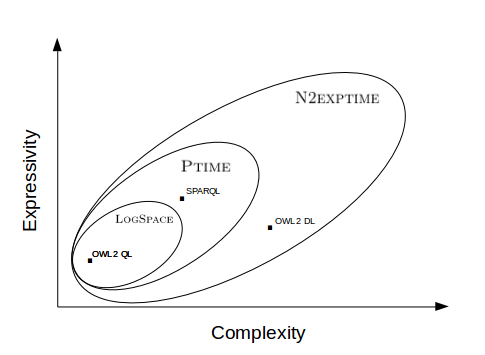
\includegraphics[width=0.95\textwidth]{complexiity_and_expressivity.png}
	\caption{Complexity and Expressivity Classes}
	\label{fig:VennDiagram}
\end{figure}
  
\begin{figure}
	\centering
		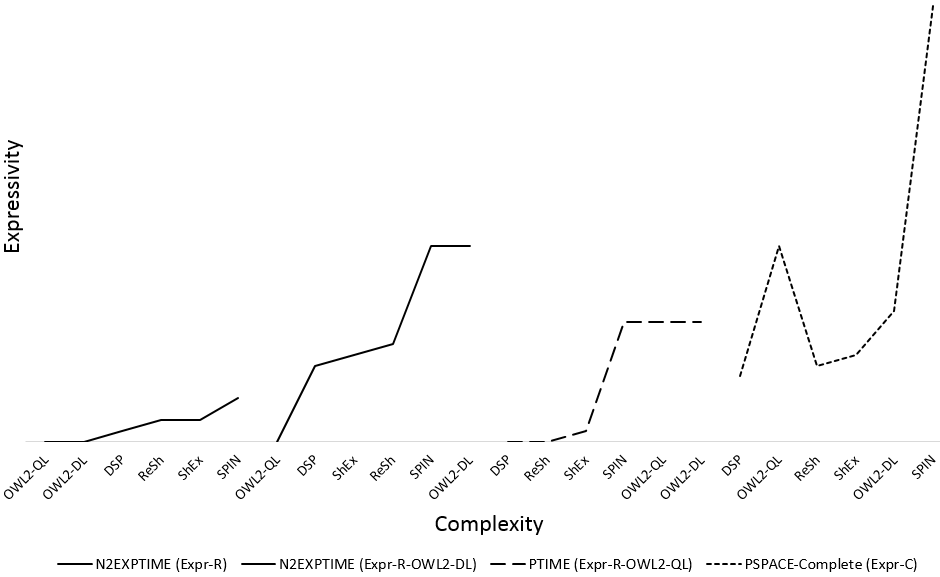
\includegraphics[width=1.00\textwidth]{expressivity-complexity-3.png}
	\caption{Expressivity and Complexity}
	\label{fig:expressivity-complexity}
\end{figure}

We assigned the five most promising DSCLs to four expressivity, four complexity, and four user-friendliness classes.
Expressivity and complexity classes can be combined in a diagram (see figure Figure~\ref{fig:expressivity-complexity}).
OWL2-DL and SPIN are the DSCLs with the highest \ms{Expr-R-OWL2-DL} to express OWL2-DL axioms in \ms{\textsc{N2exptime}}.
The highest \ms{Expr-R-OWL2-QL} expressing OWL2-QL axioms in \ms{\textsc{Ptime}} can be achieved with OWL2-QL, OWL2-DL, and SPIN.
If an application needs to cover the majority of constraints on which reasoning cannot be applied, SPIN should be used (\ms{Expr-C}) in \ms{\textsc{Pspace}-Complete}.

It depends on the individual use case, which constrains are needed to express and therefore which DSCL to choose.
As a consequence, you may select a DSCL which is not the most expressive one within one specific expressivity class, 
but may be better evaluated according to one or multiple user-friendliness classes.
If, for instance, reasoning should not be performed and three particular constraints should be covered by the DSCL.
Even if the expressivity (\ms{Expr-C}) of SPIN is much higher than of ShEx  
\begin{eqnarray*}
\ms{Expr-C}(ShEx) \subset \ms{Expr-C}(SPIN)
\end{eqnarray*}
it could be quite beneficial to choose ShEx rather than SPIN (in case the three constraints are covered by both).
Now, the user-friendliness classes comes into play:
\begin{eqnarray*}
\ms{UF-L}(SPIN) \subset \ms{UF-L}(ShEx) \\
\ms{UF-I}(SPIN) \subset \ms{UF-I}(ShEx) \\
\ms{UF-C}(SPIN) \subset \ms{UF-C}(ShEx) \\
\ms{UF-L}(ShEx) \subset \ms{UF-L}(SPIN)
\end{eqnarray*}
Although, SPIN is more adopted than ShEx, ShEx is a high-level compared to a low-level language, ShEx is more intuitive and concise than SPIN.
According to this evaluation, tools may recommend alternatives to the most expressive language SPIN.  

\section{RDF validation requirements}

\textcolor{red}{
\begin{itemize}
	\item organization according to developed classification system regarding expressivity and complexity
	\item examples for rdf constraints for each class
\end{itemize}
}

\subsection{RDF Validation Requirements and Reasoning}
\label{sec:rdf-validation-requirements-and-reasoning}

\tb{ToDO Thomas: RDF Validation Requirements and Inferencing}

\subsubsection{OWL 2 QL Reasoning}

\textbf{Subsumption}\footnote{corresponds to R-100-SUBSUMPTION}\textbf{.}
Subsumption relationships of both classes and properties are part of basic reasoning.

\begin{DL}
Jedi $\sqsubseteq$ FeelingForce \\
JediMaster $\sqsubseteq$ Jedi \\
\end{DL}

All Jedi masters are Jedis feeling the force.
These sub-class relationships can also be expressed by OWL 2 QL:

\begin{ex}
Jedi rdfs:subClassOf FeelingForce . 
JediMaster rdfs:subClassOf Jedi . 
\end{ex}

Valid data must contain the three class assignments \ms{JediMaster(Yoda)}, \ms{Jedi(Yoda)}, and \ms{FeelingForce(Yoda)}.
These class assignments can be either explicitly stated or implicitly inferred when reasoning is performed before actually validating the data.

When only the triple \ms{Yoda a JediMaster} is given and reasoning is not executed, then a constraint violation is raised.
After reasoning, however, the triples \ms{Yoda a Jedi , FeelingForce} are inferred resulting in valid data. 

\textbf{Property Domain}\footnote{corresponds to R-25-PROPERTY-DOMAIN}\textbf{.}
The property domain constraint

\begin{DL}
$\exists$ studentOf . $\top$ $\sqsubseteq$ JediStudent \\
\end{DL}

restricts that individuals having studentOf relationships must be Jedi students.
This property domain constraint can also be expressed by OWL 2 QL:

\begin{ex}
studentOf rdfs:domain JediStudent .
\end{ex}

Without reasoning, the data \ms{Anakin studentOf Obi-Wan} is invalid and causes a constraint violation, as it is not explicitly stated that \ms{Anakin} is assigned to the class \ms{Jedi}. 
When inferencing is performed before validating, the class assignment \ms{Anakin a Jedi} is inferred which prevents the constraint violation to be raised.

\subsubsection{OWL 2 DL Reasoning}

\textbf{Existential Quantification}\footnote{corresponds to R-86-EXISTENTIAL-QUANTIFICATION-ON-PROPERTIES}\textbf{.}

\begin{DL}
Jedi $\sqsubseteq$ $\exists$ hasLaserSword . LaserSword
\end{DL}

This existential quantification contains all those individuals that are connected by \ms{hasLaserSword} to an individual that is an instance of the class \ms{LaserSword}.
In OWL 2 DL, this existential quantification can also be expressed:

\begin{ex}
[ a owl:Restriction ;
  owl:onProperty hasLaserSword ;
  owl:someValuesFrom LaserSword ;
  rdfs:subClassOf Jedi ] .
\end{ex}

When our data contains the triple \ms{Luke hasLaserSword BlueLaserSword} and we perform reasoning, we can infer that \ms{Luke} is a \ms{Jedi}, as he has a laser sword.
As the individual \ms{Luke} is assigned to the class \ms{Jedi}, all constraint associated with this class are also validated, for example that Jedis must have blue laser swords.
Without reasoning, these constraints won't be validated as \ms{Luke} is not within the class extension of \ms{Jedi}.

\subsection{RDF Validation Requirements without Reasoning}

For the majority of the requirements to formulate RDF constraints, reasoning is not related to the constraints and is therefore not needed to be performed prior to validation. 
It is also possible, however, to reason before validating constraints for which reasoning does not affect validation results.
If we do reasoning by query rewriting in terms of backward chaining and if we run a constraint validation query through an engine like the --ontop-- framework\footnote{\url{http://ontop.inf.unibz.it}} or ELITE (federated query engine) \cite{nolle2013elite}, the engine will only do some rewritings if it is possible, and if you just check e.g. pattern matching there will be no rewriting.

\subsubsection{Expressible by OWL 2 QL}

\textbf{Literal Pattern Matching}\footnote{corresponds to R-44-PATTERN-MATCHING-ON-RDF-LITERALS}\textbf{.} 
\an{IMHO literal pattern matching is not expressible in DL!}\tb{but we can express it using OWL 2 DL as it is shown in the OWL 2 spec}
There are multiple use cases associated with the requirement to match literals according to given patterns.

%A social security number, for example, is a string that matches a given regular expression - which can be expressed by OWL 2 QL: 
%
%\begin{ex}
%SSN 
    %a rdfs:Datatype ;
    %owl:equivalentClass [
        %a rdfs:Datatype ;
        %owl:onDatatype xsd:string ;
        %owl:withRestrictions ( 
            %[ xsd:pattern "[0-9]{3}-[0-9]{2}-[0-9]{4}" ] ) ] .
%hasSSN rdfs:range SSN .
%\end{ex}
%
%The second axiom defines \ms{SSN} as an abbreviation for a datatype restriction on \ms{xsd:string}. 
%The first axiom explicitly declares \ms{SSN} to be a datatype. 
%The datatype \ms{SSN} can be used just like any other datatype like in the third axiom to define the range of the \ms{hasSSN} property.
%The literal pattern matching constraint above validates \ms{hasSSN} literals according to the stated regular expression causing a constraint violation for the triple 
%\ms{TimBernersLee hasSSN "123456789"\textasciicircum{}\textasciicircum{}SSN}, 
%but not for the triple \ms{TimBernersLee hasSSN "123-45-6789"\textasciicircum{}\textasciicircum{}SSN}.

Luke's droids can only have the numbers "R2-D2" or "C-3PO".
The universal restriction part of this constraint can be expressed by OWL 2 DL:
\ms{LukesDroids $\sqsubseteq$ $\forall$ droidNumber . DroidNumber}.
The restriction of the datatype \ms{DroidNumber}, however, cannot be expressed in DL, but OWL 2 QL can be used anyway:

\begin{ex}
DroidNumber 
    a rdfs:Datatype ;
    owl:equivalentClass [
        a rdfs:Datatype ;
        owl:onDatatype xsd:string ;
        owl:withRestrictions ( 
            [ xsd:pattern "R2-D2|C-3PO" ] ) ] .
\end{ex}

The second axiom defines \ms{DroidNumber} as an abbreviation for a datatype restriction on \ms{xsd:string}. 
The first axiom explicitly declares \ms{DroidNumber} to be a datatype. 
The datatype \ms{DroidNumber} can be used just like any other datatype like in the universal restriction above.
The literal pattern matching constraint validates \ms{DroidNumber} literals according to the stated regular expression causing a constraint violation for the triples 
\ms{Luke hasDroid Droideka} and \ms{Droideka droidNumber "Droideka"\textasciicircum{}\textasciicircum{}DroidNumber}, 
but not for the triples \ms{Luke hasDroid R2-D2} and \ms{R2-D2 droidNumber "R2-D2"\textasciicircum{}\textasciicircum{}DroidNumber}.

\subsubsection{Not Expressible by OWL 2 QL but by OWL 2 DL}
\label{sec:rdf-validation-requirements-without-reasoning-2}

\textbf{Allowed Values}\footnote{corresponds to R-30-ALLOWED-VALUES-FOR-RDF-OBJECTS and R-37-ALLOWED-VALUES-FOR-RDF-LITERALS}\textbf{.}
It is a common requirement to narrow down the value space of a property by an exhaustive enumeration of the valid values (both literals or resources). This is often rendered in drop down boxes or radio buttons in user interfaces. 
The constraint 'Jedis can only have blue, green, or white laser swords' can be expressed by OWL 2 DL, DSP, ReSh, ShEx, SPIN, and SPARQL.

\begin{DL}
Jedi $\equiv$ $\exists$ laserSwordColor . \{blue, green, white\} \\
\end{DL}

In DSP, the constraint does not look that concise:

\begin{ex}
personDescriptionTemplate
    a dsp:DescriptionTemplate ;
    dsp:resourceClass Jedi ;
    dsp:statementTemplate [
        a dsp:LiteralStatementTemplate ;
        dsp:property laserSwordColor ;
        dsp:literalConstraint [
            a dsp:LiteralConstraint ;
            dsp:literal "blue" ;
            dsp:literal "green" ;
            dsp:literal "white"] ] .
\end{ex}

When representing the constraint by OWL2 DL a new datatype is defined by simply enumerating its literals:

\begin{ex}
laserSwordColor rdfs:range laserSwordColors . 
laserSwordColors
    a rdfs:Datatype .
    owl:oneOf ( "blue" "green" "white" ) .
\end{ex}

Data containing the triples \ms{Yoda a Jedi ; laserSwordColor 'blue'} is valid, 
whereas data including the triples \ms{DarthMaul a Jedi ; laserSwordColor 'red'} is invalid.

\textbf{Context-Specific Exclusive OR of Properties}\footnote{corresponds to  R-11-CONTEXT-SPECIFIC-EXCLUSIVE-OR-OF-PROPERTIES}\textbf{.}
An individual can either have a relationship via property A or via property B, but not both.
To take an example, a Jedi is either attacking by sword or by force but not both (such a fight would not be fair):

\begin{DL}
Jedi $\sqsubseteq$ ($\neg$ A $\sqcap$ B) $\sqcup$ (A $\sqcap$ $\neg$ B) \\
A $\equiv$ $\exists$ attackingBySword . xsd:boolean \\
B $\equiv$ $\exists$ attackingByForce . xsd:boolean \\ 
\end{DL} 

Context-specific exclusive OR of properties can be expressed by ShEx. 
In this case, the constraint context is the class \ms{Jedi}.

\begin{ex}
Jedi { (  
    attackingBySword xsd:boolean | 
    attackingByForce xsd:boolean ) }
\end{ex}

The same constraint may be expressed by OWL 2 DL \an{Do you mean DL or QL at this point?}\tb{DisjointUnion is only supported by DL, see OWL 2 Profile spec}, but not very intuitively and concisely.
This can rather be seen as a workaround, as anonymous classes are built for each of the exclusive properties.

\begin{ex}
Jedi owl:disjointUnionOf ( CC1 CC2 ) . 
CC1 rdfs:subClassOf [
    a owl:Restriction ;
    owl:onProperty attackingBySword ;
    owl:someValuesFrom xsd:boolean ] .
CC2 rdfs:subClassOf [
    a owl:Restriction ;
    owl:onProperty attackingByForce ;
    owl:someValuesFrom xsd:boolean ] .
\end{ex}

Consider the triples \ms{Jedi(Luke)}, \ms{attackingBySword(Luke,true)}, \ms{Jedi(DarthSidious)},
\ms{attackingByForce(DarthSidious,true)}, and \ms{attackingBySword(DarthSidious,true)}
Luke as well as Darth Sidious are associated with the class \ms{Jedi}.
As Darth Sidious has both relationships, a constraint Violation is raised.

\subsubsection{Not Expressible by OWL 2 DL But by Other Constraint Languages}

The majority of constraints can neither be expressed by OWL 2 QL nor by OWL 2 DL. 
In such cases, these constraints are represented by other constraint languages like DSP, ShEx, ReSh, or SPIN.

\textbf{Default Values}\footnote{corresponds to R-31-DEFAULT-VALUES-OF-RDF-OBJECTS and R-38-DEFAULT-VALUES-OF-RDF-LITERALS}\textbf{.}
It should be possible to declare the default value for a given object and data property, e.g. so that input forms can be pre-populated and to insert a required property that is missing in a web service call. 
Siths have per default two red laser swords.
If there is only stated that Darth Maul is a Sith (\ms{DarthMaul a Sith .}), then additional default triples should be inferred: 
\ms{laserSwordColor(DarthMaul,"red")} and \ms{numberLaserSwords(DarthMaul,2)}.

The default values constraint can only be expressed by ReSh, SPIN, and SPARQL.
In SPIN, we can define a rule associated with the class \ms{owl:Thing}.
This rule is applicable for each resource, as each resource is implicitly of the type \ms{owl:Thing}. 

\begin{ex}
owl:Thing spin:rule [ a sp:Construct ; sp:text """
    CONSTRUCT {
        ?this laserSwordColor "red" ;
              numberLaserSwords 2 . }
    WHERE {             
        ?this a Sith . } """ ; ] .
\end{ex}

For each resource, the SPARQL CONSTRUCT query within the rule is executed creating the default triples.
ReSh can also be used to express default values:

\begin{ex}
Sith a ResourceShape ;
    property [
        name "laserSwordColor" ;
        propertyDefinition laserSwordColor ;
        valueType xsd:string ;
        defaultValue "red"'
        occurs Exactly-one ; ] .
\end{ex}

\section{Implementation}

SPARQL is generally seen as the method of choice to validate RDF data according to certain constraints, although it is not ideal for their formulation. 
In contrast, OWL 2 DL constraints are comparatively easy to understand, but lack an implementation to validate RDF data. 
\an{IMHO this should be described more precisely because validation in terms of inconsistency detection is still available, not sure about the completeness for OWL 2 DL}
\tb{Andy, can you write a short paragraph about inconsistency detection? Sounds interesting!}
Bosch and Eckert\cite{BoschEckert2014-2} use SPIN as basis to define a
validation environment in which the validation of any DSCL\footnote{the only limitation is that DSCLs must be represented in RDF} can be implemented by representing them in SPARQL. 
The validation implementation of DSCLs is fully declarative,
consisting of a mapping from a DSCL to SPIN in form of SPARQL CONSTRUCT queries.
SPIN represents both the SPIN mappings and the SPARQL queries in RDF. 
Within the validation environment, we fully implemented an automatic RDF validation of all OWL 2 DL\footnote{and therefore all OWL 2 QL constructs} constructs. 
\an{you should mention at this point that this validation is in terms of RDF validation, because inconsistency can't be done completely}
The implementation can be tested at \url{http://purl.org/net/rdfval-demo} and
the OWL 2 SPIN mapping is maintained at \url{https://github.com/boschthomas/OWL2-SPIN-Mapping}.

The developed DSCL classification according to the three dimensions expressivity, complexity, and user-friendliness leads to many possible extensions of the RDF validator and similar validation systems.
Users may choose if they wish to execute reasoning as a pre-validation step and which reasoning axioms they want to use to express their inference rules.
They may also select which constraints they need for their use cases.

As we defined an ordering of DSCLs for each expressivity class, we assigned reasoning axioms and constraints to complexity classes, we evaluated DSCLs regarding multiple user-friendliness criteria, the validator can provide a list of DSCLs for which the expressivity is enough to express the wished constraints and axioms.
The validator can also recommend a DSCL of that list whose user-friendliness is evaluated to be the highest according to the user-friendliness criteria.
As reasoning may cause high complexity, the validator may show which axioms from the user's selection cause the determined complexity class 
and it may provide solutions how to get to the next lower complexity class.

\section{Related Work}

\begin{itemize}
	\item See e.g. chapter 6 of Jiao Tao's dissertation - http://tw.rpi.edu/web/doc/JiaoTaoDissertation .
\end{itemize}

\textbf{CWA.}

alternate semantics for OWL (using CWA):

Several years ago Evren Siren et al proposed an alternate semantics for OWL (using CWA) so that it could be used for integrity constraint (IC) checking and this is implemented in the Stardog database. 

However, this OWL IC semantics was never submitted to a standards organization.

\begin{itemize}
	\item Clark Parsia had previously proposed the ICV semantics for OWL, but this was not submitted to W3C.
\end{itemize}

In description logics, reasoning tasks like query answering or detection of inconsistencies require the consideration of knowledge that is not only defined explicitly but also implicitly. To do so there are two different ways called forward- and backward-chaining. The first implies a materialized knowledge base, where the original knowledge base is extended by all assertions that can be inferred. State-of-the-art DL or OWL reasoners that following this approach are e.g. FaCT++ \cite{tsarkov2006fact++}, Pellet \cite{sirin2007pellet},  RacerPro \cite{haarslev2001racer}, or HermiT \cite{horrocks2012hermit}. On the second approach, the original knowledge base is kept in its original state and before queries are evaluated against the knowledge base, the queries will be rewritten such that its rewritings will consider also the implicit knowledge in the returned result set. Approaches following this way are e.g., \textsf{PerfectRef} given by Calvanese et al. \cite{Calvanese2007} or \textsf{TreeWitness} proposed by Kontchakov et al. \cite{kontchakov2011combined}. The choice between these two different ways depends on the specific application case. So the first kind is probably applied on local knowledge bases whereas the second is more appropriated for federative environments like in \cite{nolle2014efficient,nolle2013elite}.


\section{Conclusion and Future Work}

\bibliography{../../literature/literature}{}
\bibliographystyle{plain}
\setcounter{tocdepth}{1}
%\listoftodos
\end{document}
